\newpage
\section{Parsing}
\begin{itemize}
    \item Lexical Analysis: Create sequence of tokens from characters
    \item Parsing: Create abstract syntax tree from sequence of tokens
\end{itemize}

Syntax: the way in which words are put together to form phrases, clauses, or sentences

\begin{itemize}
    \item Input: sequence of tokens from lexer; 
    \item Output: parse tree of the program (But some parsers never produce a parse tree ...)
\end{itemize}

\begin{figure}[!htb]
    \centering
    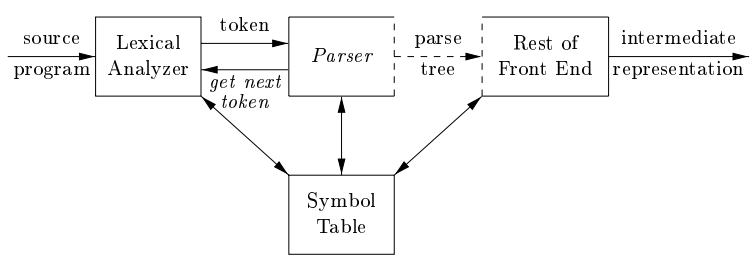
\includegraphics[width=0.42\textwidth]{pic/CP3/compiler.png}
    \caption{compiler}
\end{figure}


\subsection{Context-free Grammars}
\subsubsection{Definition for CFG}
计算理论 IV.1.

\subsubsection{Derivations}
计算理论 IV.2-3

用 CFG 生成 string

\subsubsection{Parse Trees}
计算理论 IV.5

Representing derivations as a tree. Parse trees have meaning. 

\subsubsection{Ambiguous Grammars}
A grammar is ambiguous if the same sequence of tokens can give rise to two or more parse trees.

解决二义性(Ambiguity)的方式就是重写文法. 解决二义性没有通用的方法, 一般都是通过声明 precedence(优先级) 与 associativity(结合性) 来消除文法中的二义性.

\subsubsection{End-Of-File Marker}
Use \$ to represent end of file

\subsection{Predictive Parsing}

\subsubsection{Recursive-Descent Parser}
Each grammar production turns into one clause of a recursive function. 自顶向下分析.

Problem: 预测分析需要每个子表达式的 the first terminal symbol 提供足够的信息来决定生成的是什么.

\begin{definition}[Nullable]
    Non-terminal $X$ is Nullable if $X$ can derive the empty string.
\end{definition}

\begin{definition}[First Sets]
    $First(\gamma)$ is the set of terminals that can begin strings derived from $\gamma$.
    \begin{align*}
        First(X)=\{ t|X\to^*t\alpha \}\cup\{ \epsilon | X\to^*\epsilon \}
    \end{align*}
\end{definition}
即, 如果 $X$ 可以经 0 步或多步推导出以 terminal $t$ 开头的串, 那么 $t$ 属于 ${First}(X)$;如果 $X$ 可以经 0 步或者多步推导出空串, 那么 $\epsilon$ 属于 ${First}(X)$. 

\begin{definition}[Follow Sets]
    $Follow(X)$ is the set of terminals that can immediately follow $X$. That is, $t \in Follow(X)$ if there is any derivation containing $Xt$. This can occur if the derivation contains $XYZt$ where $Y$ and $Z$ both derive $\epsilon$.
    \begin{align*}
        Follow(X)=\{ t|S\to^*\alpha Xt\beta \}
    \end{align*}
\end{definition}

$\epsilon$ 不会出现在 Follow Sets 中. Start Symbol 的 Follow Set 包含文件结束符 \$. 

\begin{algorithm}[H]
    \caption{Compute $First$, $Follow$, and $nullable$}
    \begin{algorithmic}
        \State Initialize $First$ and $Follow$ to all empty sets, and nullable to all false.
        \For{each terminal symbol $t$}
            \State $First(t)\gets \{ t \}$
        \EndFor
        \Repeat
            \For{each production $X\to Y_1Y_2\dots Y_k$}
                \For{each $i$ from $1$ to $k$, each $j$ from $i+1$ to $k$}
                    \If{all the $Y_i$ are nullable}
                        \State $nullable(X)\gets true$
                    \EndIf
                    \If{$Y_1\dots Y_{i-1}$ are all nullable}
                        \State $First(X)\gets First(X)\cup First(Y_i)$
                    \EndIf
                    \If{$Y_{i+1}\dots Y_k$ are all nullable}
                        \State $Follow(Y_i)\gets Follow(Y_i)\cup Follow(X)$
                    \EndIf
                    \If{$Y_{i+1}\dots Y_{j-1}$ are all nullable}
                        \State $Follow(Y_i)\gets Follow(Y_i)\cup First(Y_j)$
                    \EndIf
                \EndFor
            \EndFor
        \Until{$First, Follow$ and nullable didn't change in this iteration.}
    \end{algorithmic}
\end{algorithm}

\subsubsection{Building a Predictive Parser}
\begin{itemize}
    \item $Z\to XYZ | d$
    \item $Y\to c | \epsilon $
    \item $X\to a | Y$
\end{itemize}
\begin{table}[!htb]
    \centering
    \begin{tabular}[c]{cccc}\toprule
        & Nullable & First & Follow \\ \midrule
        $Z$ & no  & $d,a,c$ & \\ \cmidrule{1-1}
        $Y$ & yes & $c$ & $a,c,d $\\ \cmidrule{1-1}
        $X$ & yes & $a,c$ & $a,c,d$\\
        \bottomrule
    \end{tabular}
\end{table}


\subsubsection{Building parsing table}
\begin{itemize}
    \item if $T\in First(s)$ then enter $(X\to s)$ in row $X$, col $T$
    \item if $s$ is Nullable and $T\in Follow(X)$, enter $(X\to s)$ in row $X$, col $T$
\end{itemize}

Build parsing table where row $X$, col $T$ tells parser which clause to execute in function $X$ with next-token $T$:
\begin{table}[!htb]
    \centering
    \begin{tabular}[c]{cccc}\toprule
        & $a$ & $c$ & $d$\\ \midrule
        $Z$ & $Z\to XYZ$ & $Z\to XYZ$ &     \begin{tabular}[c]{@{}l@{}} $Z\to d$ \\ $Z\to XYZ$ \end{tabular} \\ \cmidrule{1-1}
        $Y$ & $Y\to\ $ &     \begin{tabular}[c]{@{}l@{}} $Y\to\ $ \\ $Y\to c$ \end{tabular} & $Y\to\ $ \\ \cmidrule{1-1}
        $X$ &    \begin{tabular}[c]{@{}l@{}} $X\to a$ \\ $X\to Y$ \end{tabular} & $X\to Y$ & $X\to Y$ \\ 
        \bottomrule
    \end{tabular}
\end{table}

\subsubsection{Predictive Parsing: LL(1)}
依据 grammar 构造的 parsing table 没有冲突, 此 grammar 才能被称为 LL(1) grammar.

LL(1): Left-to-right parse, Left-most derivation, 1 symbol lookahead.

In LL(k) parsing table, columns include every k-length sequence of terminals. 

用栈来存储正在生成的 parse tree, 栈顶为 leftmost non-terminal 或即将匹配的 leftmost terminal. 

\begin{example}\quad

    \begin{itemize}
        \item $E\to TX$
        \item $T\to \text{int }Y|(E)$
        \item $X\to +E|\epsilon$
        \item $Y\to *T|\epsilon$
    \end{itemize}
    \begin{table}[!htb]
        \centering
        \begin{tabular}[c]{cccc}\toprule
             & Nullable & First & Follow\\ \midrule
            $E$ & no & $(,\text{int}$ & $),$ \$  \\ \cmidrule{1-1}
            $X$ & yes & $+, \epsilon$ &  $),$ \$ \\ \cmidrule{1-1}
            $T$ & no & $(,\text{int}$ & $+,),$ \$  \\ \cmidrule{1-1}
            $Y$ & yes & $*, \epsilon$ & $+,),$ \$ \\ 
            \bottomrule
        \end{tabular}
    \end{table}

    \begin{table}[!htb]
        \centering
        \begin{tabular}[c]{ccccccc}\toprule
             & int & $*$ & $+$ & $($ & $)$ & \$ \\ \midrule
            $E$ & $TX$ & & $TX$ & & &  \\ \cmidrule{1-1}
            $X$ & & & $+E$ & & $\epsilon$ & $\epsilon$  \\ \cmidrule{1-1}
            $T$ & int $Y$ & & & $(E)$ & &  \\ \cmidrule{1-1}
            $Y$ & & $*T$ & $\epsilon$ & & $\epsilon$ & $\epsilon$  \\ 
            \bottomrule
        \end{tabular}
    \end{table}
    
    \begin{table}[!htb]
        \centering
        % \caption{}
        \begin{tabular}[c]{lll}\toprule
            Stack & Input & Action \\ \midrule
            $E$\$ & $\text{int}*\text{int}$\$ & $TX$\\
            $TX$\$ & $\text{int}*\text{int}$\$ & $\text{int }Y$\\
            $\text{int }YX$\$ & $\text{int}*\text{int}$\$ & terminal\\
            $YX$\$ & $*\text{int}$\$ & $*T$\\
            $*TX$\$ & $*\text{int}$\$ & terminal \\
            $TX$\$ & $\text{int}$\$ & int $Y$ \\
            $\text{int} YX$\$ & $\text{int}$\$ & terminal \\
            $YX$\$ & \$ & $\epsilon$ \\
            $X$\$ & \$ & $\epsilon$ \\
            \$ & \$ & Accept \\
            \bottomrule
        \end{tabular}
    \end{table}
    
\end{example}

\subsubsection{Eliminate left-recursion}
消除左递归
Rewrite the grammar so it parses the same language but the rules are different.

\begin{itemize}
    \item $E\to E+T|T \Rightarrow E\to TE', E'\to +TE'|\epsilon$
    \item $A\to A\alpha | \beta \Rightarrow A\to \beta A', A'\to \alpha A' | \epsilon$
\end{itemize}

\subsubsection{Left Factoring}
提取左因子
\begin{itemize}
    \item $E\to T+E|T \Rightarrow E\to TX, X\to +E|\epsilon$
\end{itemize}

\subsubsection{Error Recovery}
How should error be handled?
\begin{itemize}
    \item Raise an exception and quit parsing
    \item Print an error message and recover from the error
\end{itemize}
This can proceed by deleting, replacing, or inserting tokens

\subsection{LR Parsing}
\subsubsection{Bottom-up Parsing}
自底向上分析.

LL(k) 只看前面 $k$ 个 token.

LR(k): Left-to-right parse, Rightmost derivation, k-token lookahead 可以看到代表输入的全部右侧的生成.

Shift-reduce parsing:
\begin{itemize}
    \item Reduce(规约): token 到 non-terminal
    \item Shift(移进): 右移一位, 考虑下一个 terminal
\end{itemize}

LALR variant: The basis for parsers for most modern programming languages, Implemented in tools such as Yacc.

\begin{figure}[!htb]
    \centering
    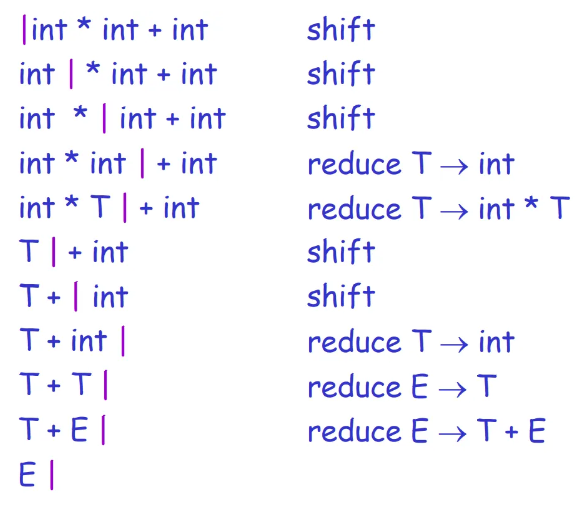
\includegraphics[width=0.309\textwidth]{pic/CP3/lrexp.png}
    \caption{Bottom-up Parsing Example}
\end{figure}

\subsubsection{LR Parsing Engine}
LR parser 使用 DFA 来决定何时 shift/reduce. 具体的:
\begin{enumerate}
    \item 通过 LR items 构造 NFA
    \item NFA 转换为 DFA
    \item DFA 转换为 LR parser table
    \item 依据 LR parser table 决定何时 shift/reduce
\end{enumerate}


一般来说, LR parser table 有以下 elements:
\begin{itemize}
    \item $s_n$: Shift into state $n$
    \item $g_n$: Goto state $n$
    \item $r_k$: Reduce by rule $k$
    \item $a$: Accept
    \item $\ $: Error 
\end{itemize}

LR parser table 具体的使用方式:
\begin{itemize}
    \item $Shift(n)$: Advance input one token; push $n$ on stack.
    \item $Reduce(k)$:
    \begin{enumerate}
        \item Pop stack as many times as the number of symbols on the right-hand side of rule $k$;
        \item Let $X$ be the left-hand-side symbol of rule $k$;
        \item Push $X$ into stack, and look up $X$ to get ``goto $n$''; 
        \item Push $n$ on top of stack.
    \end{enumerate}
    \item $Accept$: Stop parsing, report success
    \item $Error$: Stop parsing, report failure
\end{itemize}

如 \textbf{Figure} \ref{fig:explruse} 所示, stack 需要维护 token 与 state 两个量, 这里使用 (state, token) 对表示. 

\begin{algorithm}[H]
    \caption{LR parser table 使用}
    \begin{algorithmic}
        \State $a$ 表示当前入读的 token. 
        \State $a_{top}, s_{top}$ 分别为 栈顶的 token 与 state.
        \State $T_{(i,a)}$ 表示 parser table 中, state $i$ 行, token $a$ 列 所对应的 element. 
        \Repeat
            \If{$T_{(s_{top}, a)}$ is $s_n$}
                \State PUSH($n, a$)
                \State $a$=GETCHAR()
            \ElsIf{$T_{(s_{top}, a)}$ is $r_k$}
                \State Assume  rule $k$ is $A\to \beta$
                \State POP() $|\beta|$ times
                \State $T_{(s_{top}, A)}$ is $g_n$
                \State PUSH($n, A$)
            \Else
                \State Error
            \EndIf
        \Until{$T_{(s_{top}, a)}$ is accept}
        \State Accept
    \end{algorithmic}
\end{algorithm}

\quad

\quad

\quad

\begin{example}\quad
    
    \begin{enumerate}
        \item $S\to S;S$
        \item $S\to id:=E$
        \item $S\to print(L)$
        \item $E\to id$
        \item $E\to num$
        \item $E\to E+E$
        \item $E\to (S,E)$
        \item $L\to E$
        \item $L\to L, E$
    \end{enumerate}

    \begin{figure}[H]
        \centering
        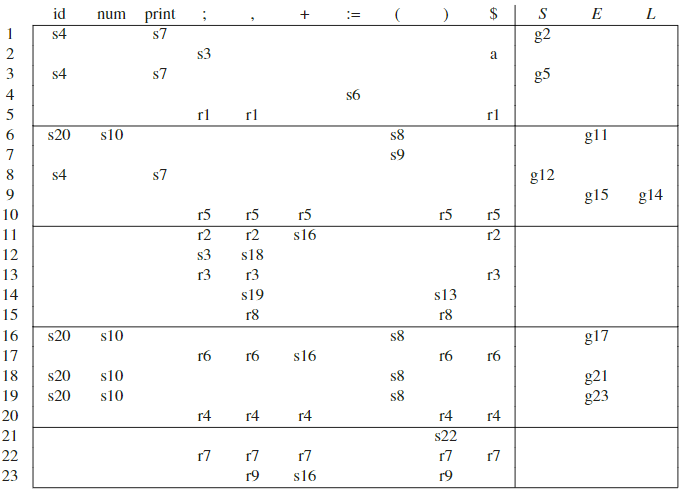
\includegraphics[width=0.42\textwidth]{pic/CP3/lrtable.png}
        \caption{LR parsing table}
    \end{figure}
    
\begin{figure}[H]
    \centering
    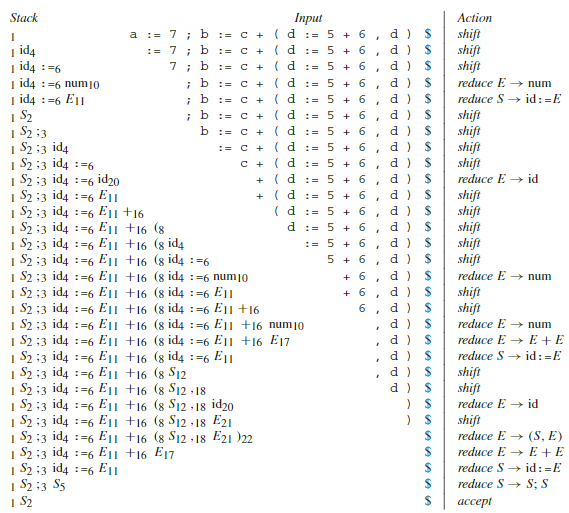
\includegraphics[width=0.42\textwidth]{pic/CP3/Shift-reduce parse of a sentence}
    \caption{Shift-reduce parse of a sentence}
    \label{fig:explruse}
\end{figure}


\end{example}

\subsubsection{LR(0) Parsing}
Making shift/reduce decisions without any lookahead.

% \begin{figure}[!htb]
%     \centering
%     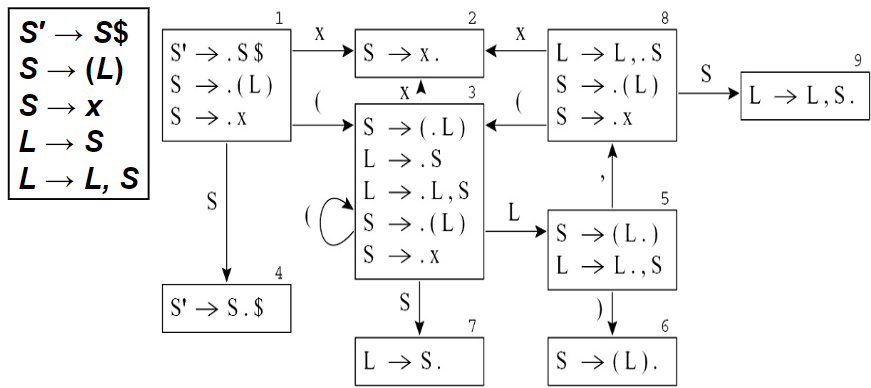
\includegraphics[width=0.42\textwidth]{pic/CP3/LR(0).png}
%     \caption{Items and States}
% \end{figure}

%TODO 完全听不懂, 回去看辅学()

\begin{definition}[LR(0) item]
    A grammar rule, combined with the dot that indicates a position in its right-hand side, is called an item (specifically, an LR(0) item).
\end{definition}

A state is just a set of items.

\begin{example}\label{exp:lr0}
    For grammar
    \begin{enumerate}
        \item $S'\to S$
        \item $S\to (S)S$
        \item $S\to \epsilon$
    \end{enumerate}
    The LR(0) items include:
    \begin{itemize}
        \item $S'\to .S$, $S'\to S.$
        \item $S\to .(S)S$, $S\to (.S)S$, $S\to (S.)S$, $S\to (S).S$, $S\to (S)S.$
        \item $S\to .\epsilon$, $S\to \epsilon.$
    \end{itemize}
\end{example}

LR(0) Item  之间存在一些转换关系:
\begin{itemize}
    \item $X\to .\alpha\beta$, 接受 $\alpha$ 变为 $X\to \alpha . \beta$
    \item 若有 $X\to \gamma T\omega, Y\to \alpha\beta$, 则 $X\to \gamma . Y \omega$ 可以转换为 $Y\to .\alpha \beta$ (因为凑 $X$ 必须先凑 $Y$)
\end{itemize}
通过这些转换关系将 LR(0) items 写为一个 NFA, 然后将 NFA 转换为 DFA. 

% \begin{figure}[!htb]
%     \centering
%     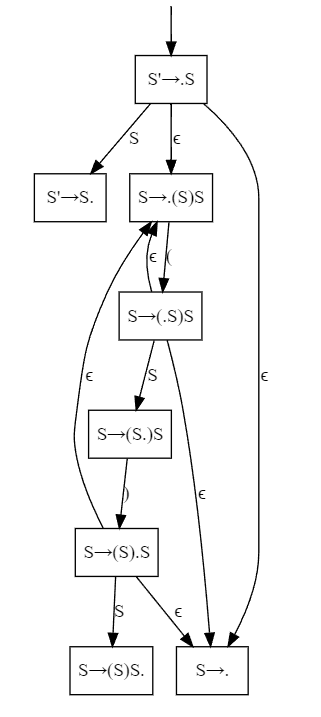
\includegraphics[width=0.22\textwidth]{pic/CP3/expnfa.png}
%     \caption{NFA for \textbf{Example} \ref{exp:lr0}}
% \end{figure}

\begin{figure}[!htb]
    \centering
    \begin{subfigure}{0.22\textwidth}
        \centering
        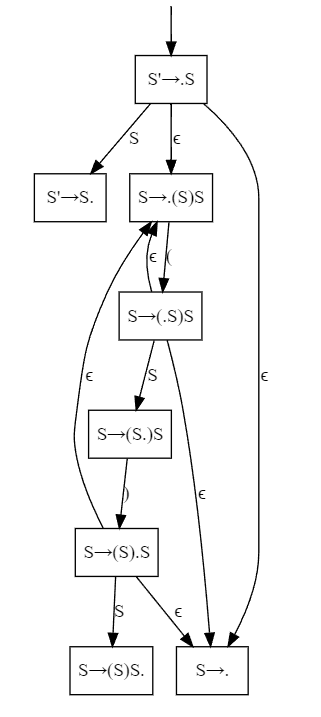
\includegraphics[height=2\textwidth]{pic/CP3/expnfa.png}
        \caption{NFA}
    \end{subfigure}
    \begin{subfigure}{0.22\textwidth}
        \centering
        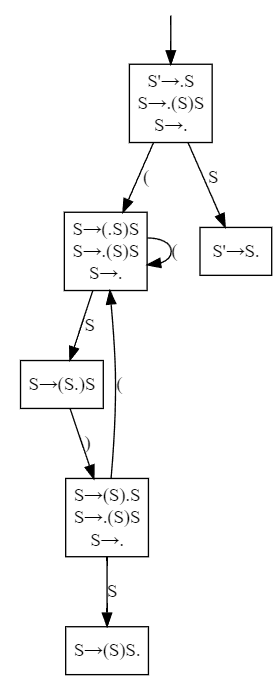
\includegraphics[height=2\textwidth]{pic/CP3/expdfa.png}
        \caption{DFA}
    \end{subfigure}
    \caption{LR(0) NFA and DFA for \textbf{Example} \ref{exp:lr0}}
\end{figure}


然后依据 DFA 与 如下规则:
\begin{itemize}
    \item 对每条 $t$ 是 terminal 的边 $S_i \overset{t}{\rightarrow} S_j$, 令 $T_{(i,t)}$ 为 $s_j$. 其中, $S_i$ 表示状态 $i$,
    \item 对每条 $X$ 是 non-terminal 的边 $S_i \overset{X}{\rightarrow} S_j$, 令 $T_{(i,X)}$ 为 $g_j$.
    \item 对每个包含 $X\to \gamma.$ (结尾带点的规则 $k$) 的状态 $i$, 对每个 terminal $t$, 令 $T_{(i,t)}$ 为 $r_k$.
    \item 对每个包含 $S'\to S.\$ $ 的状态 $i$, 令 $T_{(i,\$)}$ 为 accept.
\end{itemize}

这样就可以构造出 LR(0) Parsing Table, 如 \textbf{Table} \ref{tab:explr0} 所示. 

注意到 $T_{(1,()}, T_{(3,()}, T_{(5,()}$ 出现了冲突, 这三个都属于 shift-reduce conflict. 只有构造出的 LR(0) Parsing Table 没有冲突时, grammar 才能被称为 LR(0) grammar.

\begin{table}[!htb]
    \centering
    \caption{LR(0) Parsing Table for \textbf{Example} \ref{exp:lr0}}
    \label{tab:explr0}
    \begin{tabular}[c]{cccc|c}\toprule
         & ( & ) & \$ & $S$\\ \midrule
        1 & $s_3, r_3$ & $r_3$ & $r_3$ & $g_2$\\ \cmidrule{1-1}
        2 & $r_1$ & $r_1$ & $r_1$, accept & \\ \cmidrule{1-1}
        3 & $s_3, r_3$ & $r_3$ & $r_3$ & $g_4$\\ \cmidrule{1-1}
        4 & & $s_5$ & & \\ \cmidrule{1-1}
        5 & $s_3, r_3$ & $r_3$ & $r_3$ & $g_6$\\ \cmidrule{1-1}
        6 & $r_2$ & $r_2$ & $r_2$ & \\
        \bottomrule
    \end{tabular}
\end{table}


\subsubsection{SLR Parsing}
SLR 中的 S 表示 Simple. SLR Parsing 在 LR(0) 的基础上通过简单的判断尝试解决冲突.

SLR 在构造形如 LR(0) 的 DFA 之上, 还需要计算每个 non-terminal 的 Follow Set. SLR 只对那些下一个符号在对应 non-terminal 的 Follow Set 的情况进行 reduc. 具体更改如下:
\begin{itemize}
    \item 对每个包含 $X\to \gamma.$ (结尾带点的规则 $k$) 的状态 $i$, 对每个 terminal $t\in Follow(X)$, 令 $T_{(i,t)}$ 为 $r_k$.
\end{itemize}

构造出的 SLR Parsing Table, 如 \textbf{Table} \ref{tab:expslr1} 所示.

\begin{table}[!htb]
    \centering
    \caption{SLR Parsing Table for \textbf{Example} \ref{exp:lr0}}
    \label{tab:expslr1}
    \begin{tabular}[c]{cccc|c}\toprule
         & ( & ) & \$ & $S$\\ \midrule
        1 & $s_3$ & $r_3$ & $r_3$ & $g_2$\\ \cmidrule{1-1}
        2 & & & $r_1$, accept & \\ \cmidrule{1-1}
        3 & $s_3$ & $r_3$ & $r_3$ & $g_4$\\ \cmidrule{1-1}
        4 & & $s_5$ & & \\ \cmidrule{1-1}
        5 & $s_3$ & $r_3$ & $r_3$ & $g_6$\\ \cmidrule{1-1}
        6 & & $r_2$ & $r_2$ & \\
        \bottomrule
    \end{tabular}
\end{table}

\subsubsection{LR(1) Parsing}
\begin{definition}
    An LR(1) item consists of a grammar production, a right-hand-side position (represented by the dot), and a lookahead symbol. The idea is that an item ($A \to \alpha.\beta, x$) indicates that the sequence $\alpha$ is on top of the stack, and at the head of the input is a string derivable from $\beta x$.
\end{definition}

LR(1) Item 存在如下两种转化:
\begin{itemize}
    \item $X\to .\alpha\beta, t$ 接受 $\alpha$ 变为 $X\to \alpha . \beta, t$ 
    \item 若有 $X\to \gamma T\omega, Y\to \alpha\beta$, 则对于每个 $t_i\in First(\omega t)$ ($\omega$ 可以是 $\epsilon$),  $X\to \gamma . Y \omega, t$ 可以转换为 $Y\to .\alpha \beta, t_i$
\end{itemize}

\begin{example}\label{exp:lr1}
    对于如下 grammar:
    \begin{itemize}
        \item $S'\to S$
        \item $S \to aAd$
        \item $S \to bBd$
        \item $S \to aBe$
        \item $S \to bAe$
        \item $A \to c$
        \item $B \to c$
    \end{itemize}
    Start Symbol 有 LR(1) Item $S'\to .S, \$ $
    
    \begin{figure}[!htb]
        \centering
        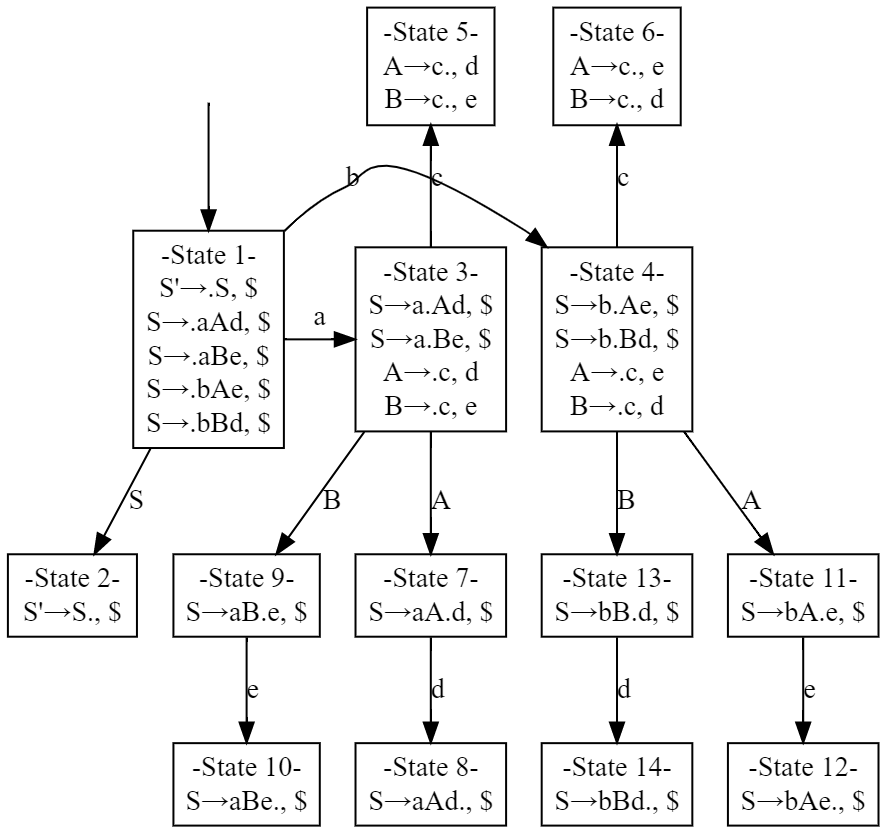
\includegraphics[width=0.42\textwidth]{pic/CP3/explr1dfa.png}
        \caption{LR(1) DFA for \textbf{Example} \ref{exp:lr1}}
        \label{fig:explr1}
    \end{figure}
    
\end{example}

构造 LR(1) Parsing Table 的方式, 也是只基于 LR(0) 更改了 reduce:
\begin{itemize}
    \item 对每个包含 $X\to \gamma.$ (结尾带点的规则 $k$) 的状态 $i$, 对每个 lookahead symbol $t$, 令 $T_{(i,t)}$ 为 $r_k$.
\end{itemize}

\subsubsection{LALR(1) Parsing}
LALR(1)(Look-Ahead LR(1)) 是 LR(1) 的简化版本. 

对于每一个状态, 将其包含的所有 LR(1) items 的第一个分量的集合称为这个状态的核心 (core). 

例如, 对于 \textbf{Figure} \ref{fig:explr1}, 其状态 5 和 6 的核心均为 $\{A\to c., B\to c.\}$. 将这样的具有相同核心的状态进行合并, 通常能够减少许多状态. 

但是, 这有时(虽然很少)也可能引入 reduce-reduce conflict. 不过问题不大. 

\begin{figure}[!htb]
    \centering
    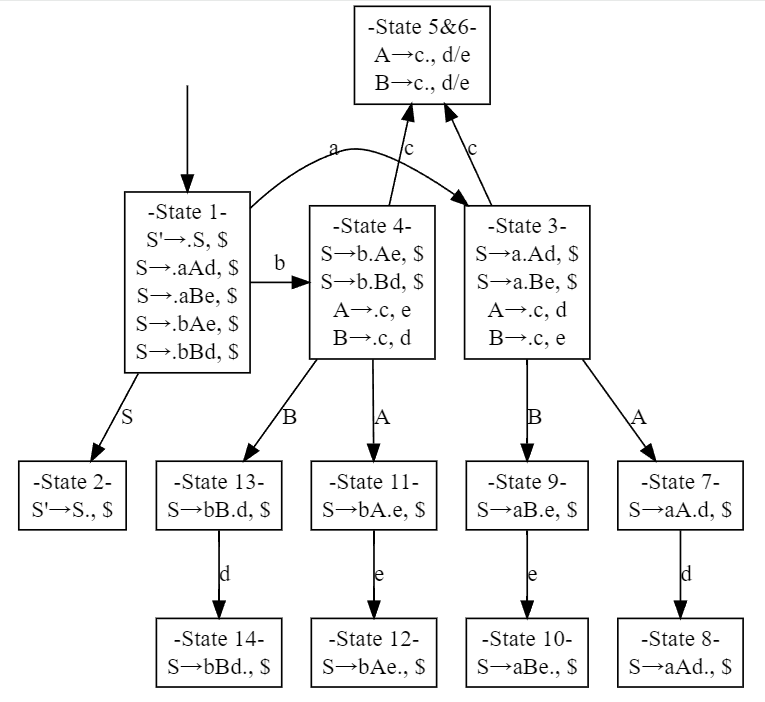
\includegraphics[width=0.42\textwidth]{pic/CP3/explalr1dfa.png}
    \caption{LALR(1) DFA for \textbf{Example} \ref{exp:lr1}}
\end{figure}

\subsubsection{Hierarchy of Grammar Classes}
The relationship between several classes of grammars. 
\begin{figure}[!htb]
    \centering
    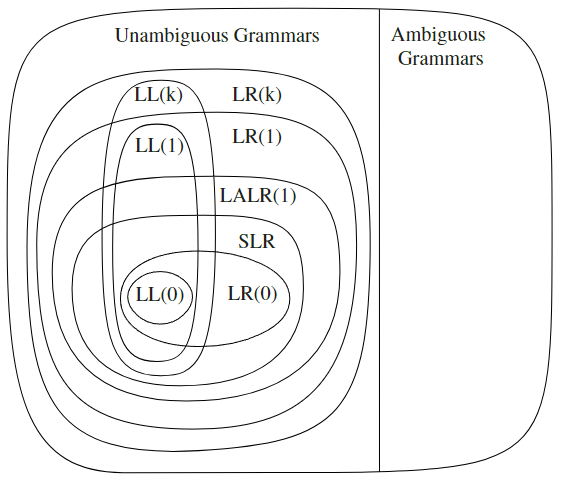
\includegraphics[width=0.309\textwidth]{pic/CP3/A hierarchy of grammar classes.}
    \caption{A hierarchy of grammar classes.}
\end{figure}

\subsection{Using Parser Generators}
\subsubsection{Yacc}
Yacc (``Yet another compiler-compiler''): A classic and widely used parser
generator

A Yacc specification is divided into three sections, separated by \%\% marks:

\begin{minted}{c}
    parser declarations
    %%
    grammar rules
    %%
    programs
\end{minted}

\begin{itemize}
    \item Parser declaration: a list of $N, T$ and so on
    \item Programs: ordinary C code usable from the semantic action
    \item Grammar rules: production of the form
    \subitem \mintinline{c}{exp: exp PLUS exp {semantic action}}  
    \subitem where \mintinline{c}{exp} is a nonterminal producing a right-hand side of \mintinline{c}{exp + exp}, and \mintinline{c}{PLUS} is a terminal symbol (token). The semantic action is written in ordinary C and will be executed whenever the parser reduces using this rule.
\end{itemize}

\begin{example}
    For grammar
    \begin{enumerate}
        \item $P \to L$
        \item $S \to id := id$
        \item $S \to$ while $id$ do $S$
        \item $S \to$ begin $L$ end
        \item $S \to$ if $id$ then $S$
        \item $S \to$ if $id$ then $S$ else $S$
        \item $L \to S$
        \item $L \to L ; S$
    \end{enumerate}

    \begin{minted}{c}
%{
int yylex(void);
void yyerror(char *s) { EM_error(EM_tokPos, "%s", s); }
%}
%token ID WHILE BEGIN END DO IF THEN ELSE SEMI ASSIGN
%start prog
%%
prog: stmlist
stm : ID ASSIGN ID
    | WHILE ID DO stm
    | BEGIN stmlist END
    | IF ID THEN stm
    | IF ID THEN stm ELSE stm
stmlist : stm
        | stmlist SEMI stm
    \end{minted}
    
\end{example}

\subsubsection{Conflicts}
\begin{itemize}
    \item shift-reduce conflict: Resolved using shift by default in Yacc
    \item reduce-reduce conflict: Resolved using the rule appears early in the grammar
\end{itemize}

\subsubsection{Precedence Directives}
Ambiguous grammars are still be useful if finding ways to resolve the conflict.

Yacc uses precedence directives to resolve this class of shift-reduce conflicts

\subsection{Error Recovery}
\subsubsection{Recovery Using the Error Symbol}
Local error recovery mechanisms.

If a syntax error is encountered in the middle of an expression, the parser should skip to the next semicolon or right parenthesis(called synchronizing tokens) and resume parsing.

error is considered a terminal symbol. When the LR parser reaches an error state, it takes the following actions:
\begin{enumerate}
    \item Pop the stack (if necessary) until a state is reached in which the action for the error token is shift.
    \item Shift the error token.
    \item Discard input symbols (if necessary) until a lookahead is reached that has a nonerror action in the current state.
    \item Resume normal parsing.
\end{enumerate}

\subsubsection{Global Error Repair}
Global error repair: finds the smallest set of insertions and deletions that would turn the source string into a syntactically correct string, even if the insertions and deletions are not at a point where an LL or LR parser would first report an error.

Burke-Fisher error repair: single-token insertion, deletion, or replacement at every point that occurs no earlier than $K$ tokens before the point where the parser reported the error.